% Short demo for \LaTeX beamer theme with ACON style layout
%
% Author: Thomas Meurer <tm@tf.uni-kiel.de>
% Version history:
% v0 ... 2016/12/09

\documentclass[10pt,t,aspectratio=1610]{beamer}
%\usetheme[german]{ACON} %or 
\usetheme{ACON}

% We define  a command \sfcite which enables to add citations but to
% preserve the citation number throughout the presentation. Citations
% are placed on the slide, where \sfcite is called. For the standard
% behavior of citations use \footcite.
%
% This also requires to add the following two lines to the main LaTeX
% source file:
%
\usepackage[style=numeric-comp,citetracker=true,sorting=none]{biblatex}
\bibliography{example}
\usepackage{abbreviations} %Provide an abbreviations file if equations
                          %are used
\usepackage{curve2e}

\usepackage{media9} %For Video Playback

% =======================

% If the title exceeds two lines then adjust the title font size 
%\setbeamerfont{title}{series=\bfseries,size={\fontsize{18}{18}}}

% =======================

\title{Eine Anwendung des Reinforcement Learning zur Regelung dynamischer Systeme}
\subtitle{Abschlussvortrag Bachelorarbeit}
\author[J. Wilinski]{Jonas Helmut Wilinski}
\pauthoremail{stu118261@mail.uni-kiel.de}
\institute[ACON]{Abschlussvortrag Bachelorarbeit, Kiel (Germany),}
\date{14. September 2018}
\begin{document}

% =======================

\begin{frame}[plain]
  \titlepage
\end{frame}

% =======================

\begin{frame}
	\frametitle{Grundlagen biologischer neuronaler Netze}
	\framesubtitle{Der \glqq Touch Withdrawal Circuit\grqq{} des C.Elegans}
	
	
\end{frame}

% =======================

\begin{frame}
	\frametitle{Bisherige Schritte}
	\framesubtitle{Implementierung des \btEmph{Neuronalen Netzes}}
	
		\begin{itemize}
			\item Implementierung durch Nutzung von Transitionsmatrizen $A, A_{Gap}, B, B_{Gap}$ um die Verbindungen zwischen Neuronen darzustellen
			\item Parameter $U_{Leak}, w, \sigma, C_m, G_{Leak}$ sind ebenfalls anhand der Transitionsmatrizen angeordnet
			\item Das \texttt{compute}-Modul berechnet durch die Modellgleichungen die Ströme der Synapsen bzw. Gap-Junctions und folglich die Membranpotentiale der Neuronen
			\item Somit kommt es zu Fire-Ereignissen und die Motor-Neuronen werden angeregt
		\end{itemize}
		
		\begin{center}
			\centering
			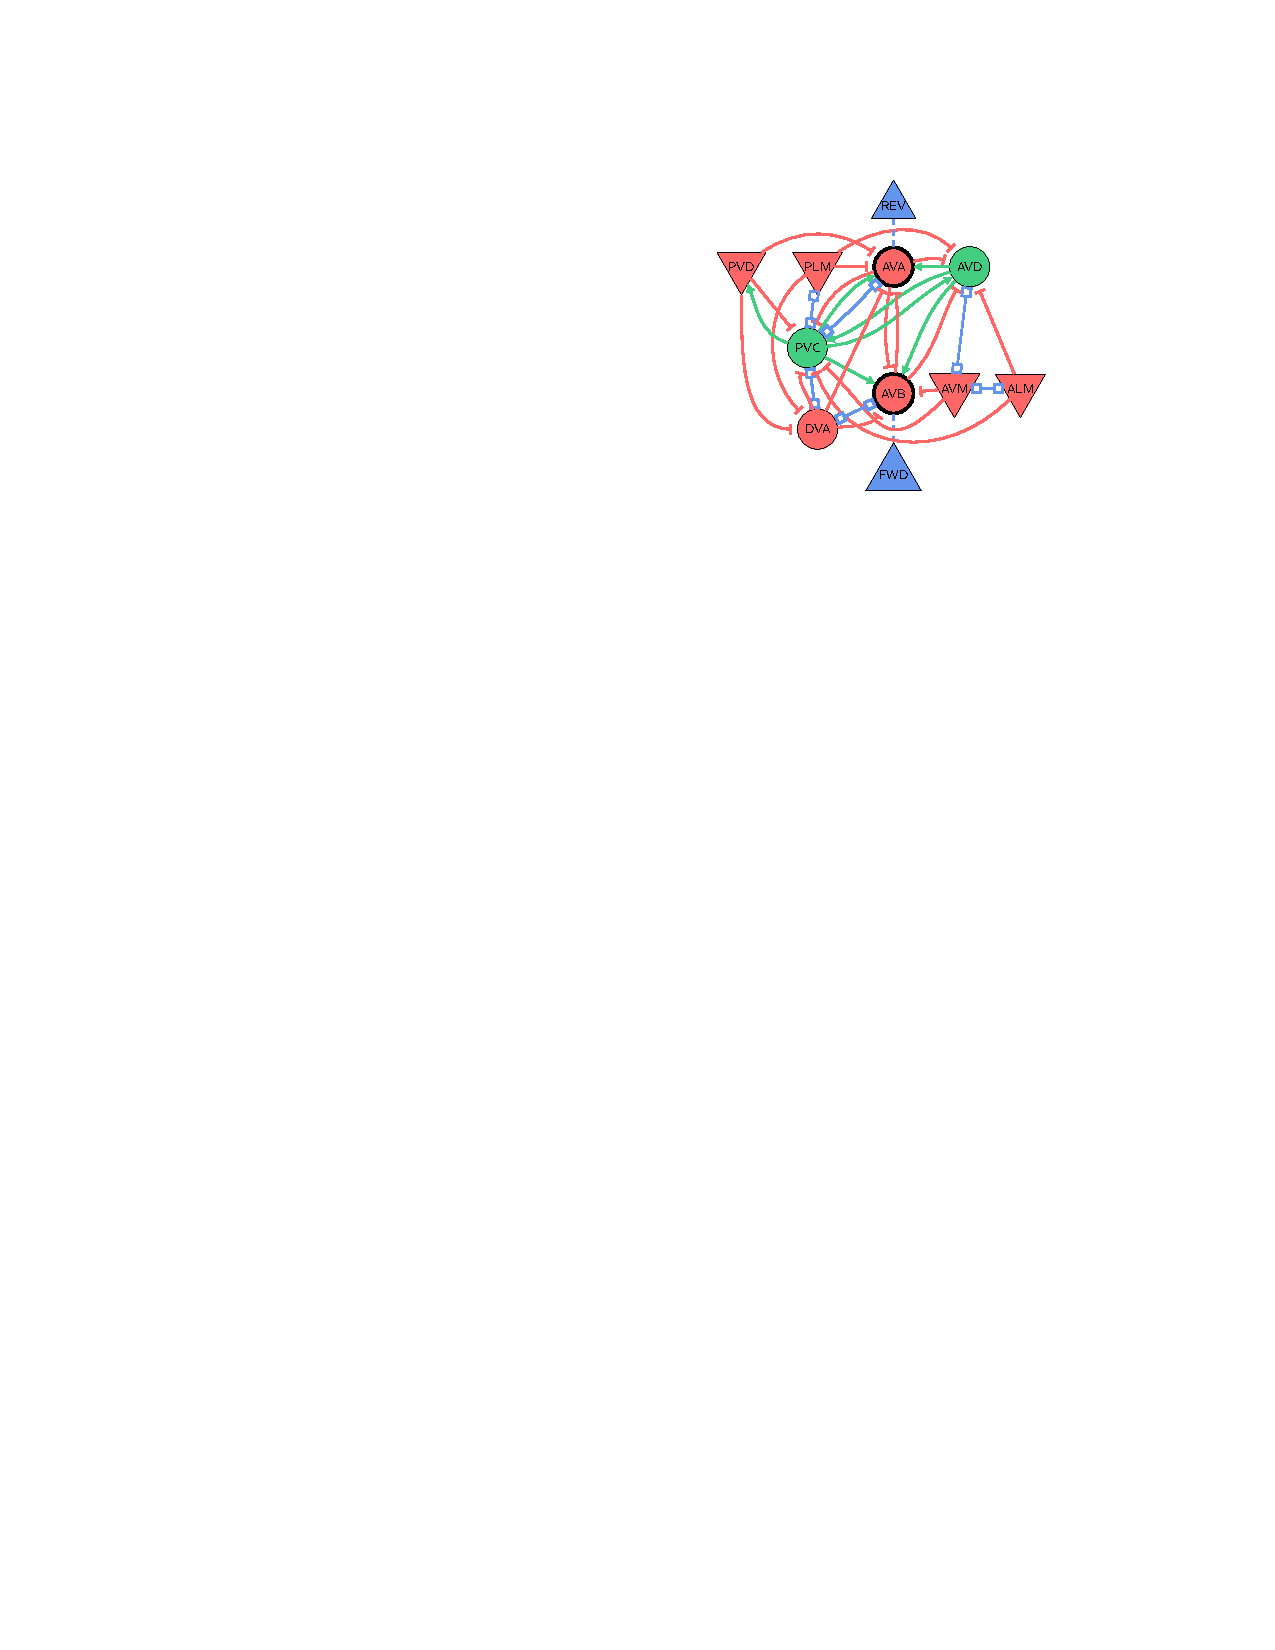
\includegraphics[width=4.6cm]{figures/Orig_TW_Circuit.pdf}
			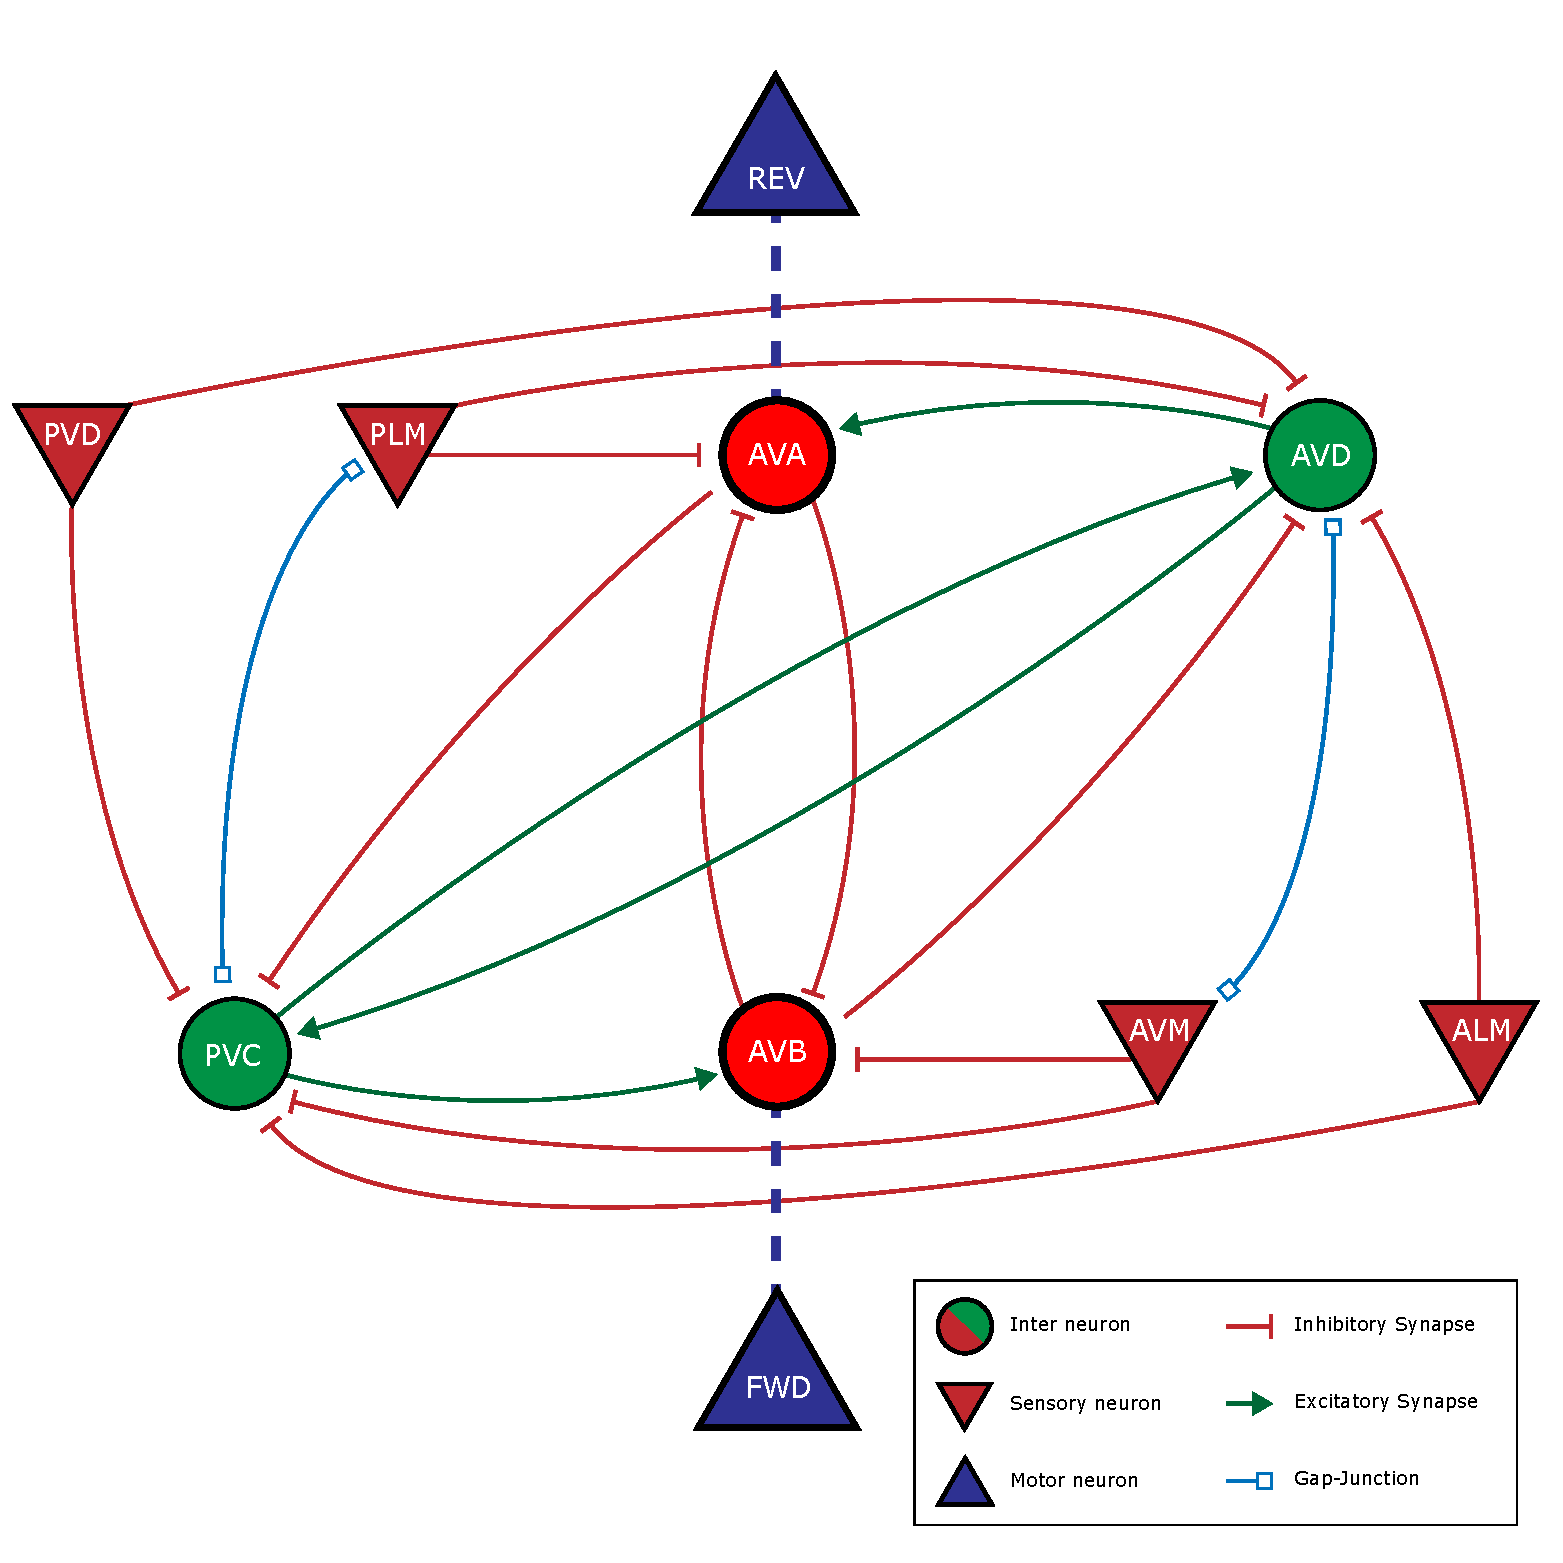
\includegraphics[width=4.8cm]{figures/Neural_Net_v3_plain.pdf}
		\end{center}
\end{frame}

% =======================

\begin{frame}
  \frametitle{Formatting text}
  \framesubtitle{Color and thickness}

  \begin{itemize}
  \item Emphasizing text  cell
    \begin{itemize}
    \item \texttt{\textbackslash cEmph} provides \cEmph{this text}
    \item \texttt{\textbackslash ctEmph} provides \ctEmph{this text}
    \item \texttt{\textbackslash tEmph} provides \tEmph{this text}
    \item \texttt{\textbackslash bEmph} provides \bEmph{this text}
    \item \texttt{\textbackslash btEmph} provides \btEmph{this text}
    \end{itemize}
  \end{itemize}  
\end{frame}

% =======================

\begin{frame}
	\frametitle{Reinforcement Learning}
	\framesubtitle{Lernen mit Belohnung}


\end{frame}

% =======================

\begin{frame}
	\frametitle{OpenAI Gym}
	\framesubtitle{Die \texttt{CartPole\_v0} Umgebung}


\end{frame}

% =======================

\begin{frame}
	\frametitle{Animation des inversen Pendels}
	\framesubtitle{Parametersuche durch RandomSearch}
	
	\includemedia[
	width=0.4\linewidth,
	totalheight=0.225\linewidth,
	activate=pageopen,
	passcontext,  %show VPlayer's right-click menu
	addresource=video/20180830_Render.mp4,
	flashvars={
		%important: same path as in `addresource'
		source=video/20180830_Render.mp4
	}
	]{\fbox{PLAY}}{VPlayer.swf}


\end{frame}

% =======================

\begin{frame}[fragile]
  \frametitle{Boxes}
  \framesubtitle{Some examples}

\begin{verbatim}
\begin{displaybox}{0.995\textwidth}
  Example 1: use 0.995\textbackslash textwidth for full width box  
\end{displaybox}
\end{verbatim}
  
  \begin{displaybox}{0.995\textwidth}
    % 
    Example 1: use 0.995\textbackslash textwidth for full width box 
    % 
  \end{displaybox}
  
\begin{verbatim}
\begin{alignbox}{0.75\textwidth} 
  Use for math related environments including text line (blank line below)

  \begin{align}
    y = x^2
  \end{align}
\end{alignbox}
\end{verbatim}
  
  \begin{alignbox}{0.75\textwidth}
    Use for math related environments including text line (blank line below)
    
    \begin{align}
      y = x^2
    \end{align}
  \end{alignbox}
  %
\end{frame}

% =======================

\begin{frame}[fragile,fragile]
  \frametitle{Boxes}
  \framesubtitle{Some examples}
  
\begin{verbatim}
\begin{alignbox}{0.5\textwidth} 
  \begin{align}
    y = x^2
  \end{align}
\end{alignbox}
\end{verbatim}
  
  \begin{alignbox}{0.5\textwidth}
    \begin{align}
      y = x^2
    \end{align}
  \end{alignbox}
  %

\begin{verbatim}
This shows the use of an \texttt{inlinebox} environment
\begin{inlinebox}{1cm}
  abc
\end{inlinebox}
\end{verbatim}\newenvironment{onlinebox}[1]

This shows the use of an \texttt{inlinebox} environment
\begin{inlinebox}{1cm}
  abc
\end{inlinebox}

\end{frame}

% =======================

\begin{frame}\frametitle{Differenzielle Flachheit}
  \framesubtitle{Inversionsbasierte Trajektorienplanung}
  %
  \newcommand{\pfeil}{\VECTOR(0,0)(3,0)}
  \newcommand{\kasten}{\polyline(0,0)(4,0)(4,3)(0,3)(0,0)}
  %
  \begin{itemize}
  \item \btEmph{Differenzielle Flachheit}\sfcite{fliess:95}
    \medskip
    \begin{inlinebox}{0.925\textwidth}
      Ein System $\dot{\xv[]}=\bs{f}(\xv[],\uv[])$ wird \tEmph{differenziell
        flach} genannt, wenn ein so genannter \tEmph{flacher Ausgang}
      $\yv[]=\bs{h}(\xv[],\uv[])$, $\dim\yv[]=\dim\uv[]$ existiert, so dass \\[1ex]
      % 
      \phantom{-----} 
      $\xv =
      \bs{\theta_{\xv[]}}\Bigl(\yv[],\dot{\yv[]},\ldots,\yv[^{(\beta)}]\Bigr)$,
      \qquad 
      $\uv =
      \bs{\theta_{\uv[]}}\Bigl(\yv[],\dot{\yv[]},\ldots,\yv[^{(\beta+1)}]\Bigr)$.
    \end{inlinebox}
    %
    $\Rightarrow$ \tEmph{Differenzielle Zustands-- und
      Eingangsparametrierung} \pause\\[-1ex]
    % 
    \unitlength0.5cm
    \begin{picture}(26,4)(0,1.25)
      \linethickness{1.25pt}
      \put(1,0){%
        \put(10,3){\pfeil}
        \put(13,1.5){\kasten}
        \put(13.75,2.75){System}
        \put(17,3){\pfeil}
        % 
        \put(17.5,3.5){$\xv[\cts]\to\cEmph{\xvd[\cts]=\bs{\theta_{\xv[]}}\bigl(\yvd[],\dot{\yvd[]},...\bigr)}$}
      }
      %
      \put(3,3){\cEmph{\pfeil}}
      \put(6,1.5){\cEmph{\kasten}}
      \put(10,3){\Line(0,0)(0,0)(1,0)}
      \put(6.15,2.75){$\bs{\theta}_{\uv[]}\bigl(\yvd[],\!\dot{\yvd[]}\!,...\bigr)$}
      \put(10.1,3.5){$\cEmph{\uvd}=\uv$}
      \put(3.25,3.5){\cEmph{$\yvd$}}
    \end{picture}\pause\\
    %
    $\Rightarrow$ Methodische \"Ubertragung auf
    \tEmph{verteilt--parametrische Systeme}
  \end{itemize}
  % 
\end{frame}

% =======================

\ClosingSlide

\end{document}

%%% Local Variables:
%%% mode: latex
%%% TeX-master: t
%%% End:
